\chapter{Term Analysis}
\label{cha:analysis}
In this chapter, we mainly focus on recognizing the reasons that standard IR methods fail when the relevant patent documents are complete and in English. In fact, we will investigate the problem from term analysis point of view for both patent query and relevant documents because we are interested in finding what is wrong in term matching process between a patent query and relevant patents. 

%%%%%%%%%%%%%%%%%%%%%%%%%%%%%%%%%%%%%%%%%%%%%%%%%%%%%%%%%%%%%%
%%%%%%%%%%%%%%%%%%%%%%%% SECTION 1 %%%%%%%%%%%%%%%%%%%%%%%%%%
%%%%%%%%%%%%%%%%%%%%%%%%%%%%%%%%%%%%%%%%%%%%%%%%%%%%%%%%%%%%%%

\section{Term Mismatch}
\label{sec:termmismatch}
%\input{TermAnalysis/termmismatch}
Standard retrieval models rank documents based on term matching process between the query and documents. Previous works complain about a significant term mismatch between the query patent and relevant patents~\citep{roda2010clef}~\citep{magdy2012toward}. To discover the relation between the term overlap and retrievablity, we calculate the average term overlap per query for retrieved relevant patents (TPs), retrieved non-relevant patents (FPs), and non-retrieved relevant patents (FNs) respectively as follows:    
%%%%%%%%%%%%%%%%%%%%%%%%%%%%%%%%%%%%%%%%%%%%%%%%%%%%%%%%%%%%%%
\begin{equation} 
\mbox{Avg. term overlap per query } = \frac{1}{|D|}\sum_{d\in D}\frac{|terms_{Q\cap d}|}{|Q|}
\label{eq:fntermoverlap}
\end{equation}
%\vspace*{-1ex}
%\begin{displaymath}t\in \lbrace \mbox{terms in top-100 retrieved documents}\rbrace\end{displaymath}
%%%%%%%%%%%%%%%%%%%%%%%%%%%%%%%%%%%%%%%%%%%%%%%%%%%%%%%%%%%%%%

Where, $D$ is the number of TPs, FPs, or FNs for each query respectively, $ |terms_{Q\cap d}| $ is the number of query terms appear in each TP/FP/FN patent, $ |Q| $ is the size of the query.

The results (Figure~\ref{fig:overlap}) illustrate two main facts:
\begin{enumerate}
\item The majority of patent documents (about 94\%) are retrieved  (TPs and FPs) when they have a term overlap with a query above $ 0.2 $.
\item There is sufficient term overlap with the query for FN patents too, though compared to TPs and FPs, more patent documents can be seen with the overlap less than $ 0.2 $ (about 24\%).  
\end{enumerate}
 
%%%%%%%%%%%%%%%%%%%%%%%%%%%%%%%%%%%%%%%%%%%%%%%%%%%%%%%%%%%%%%
\begin{figure}[t!]
\begin{centering}
\subfigure[Query and TP patents.]{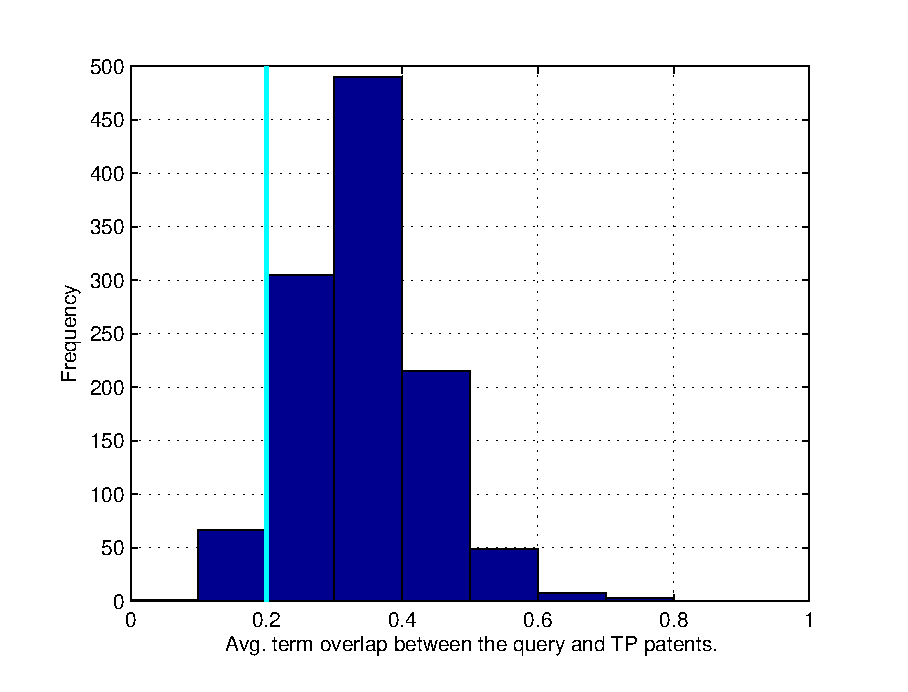
\includegraphics[width=5cm]{figs/olap-tps-all.eps}}\subfigure[Query and FP patents.]{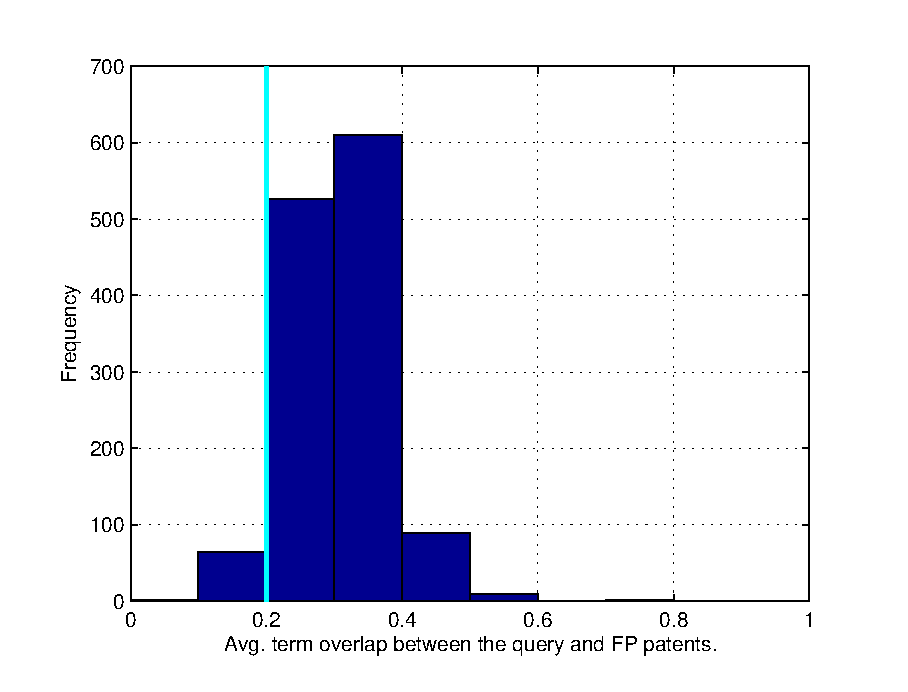
\includegraphics[width=5cm]{figs/olap-fps-all.eps}}\subfigure[{Query and FN patents.}]{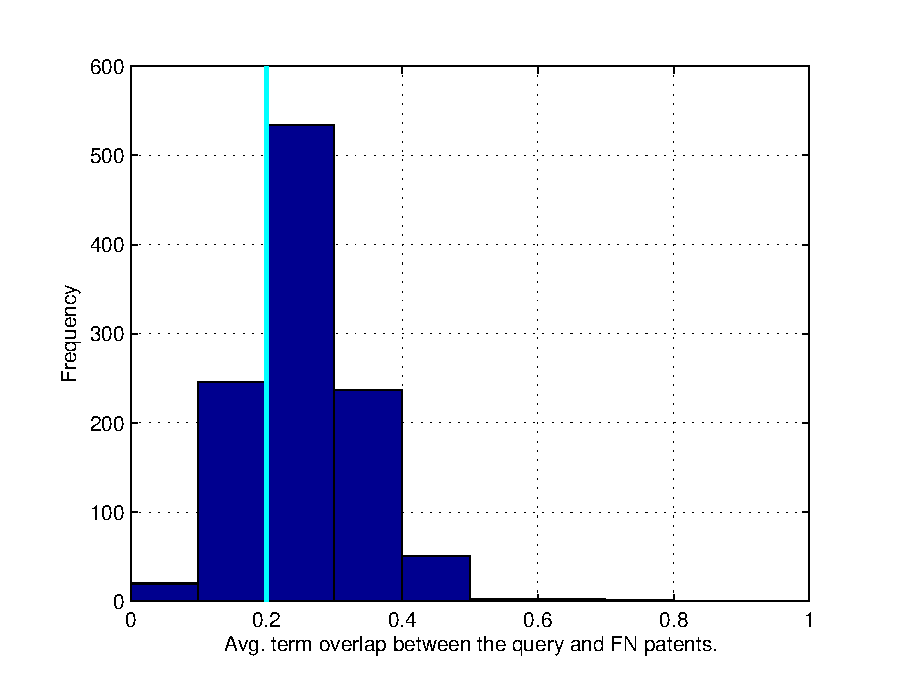
\includegraphics[width=5cm]{figs/olap-fns-all.eps}}
\par\end{centering}

\protect\caption{The distribution of term overlap between the query and documents over 1303 test queries.}
\label{fig:overlap}
\end{figure}
%%%%%%%%%%%%%%%%%%%%%%%%%%%%%%%%%%%%%%%%%%%%%%%%%%%%%%%%%%%%%%
Therefore, we conclude that reasons beyond low or zero term match are involved in low retrieval effectiveness.   

%%%%%%%%%%%%%%%%%%%%%%%%%%%%%%%%%%%%%%%%%%%%%%%%%%%%%%%%%%%%%%
%%%%%%%%%%%%%%%%%%%%%%%%% SECTION 2 %%%%%%%%%%%%%%%%%%%%%%%%%%
%%%%%%%%%%%%%%%%%%%%%%%%%%%%%%%%%%%%%%%%%%%%%%%%%%%%%%%%%%%%%%
\section{Oracular Relevance Feedback System}
In this section, we develop an oracular relevance feedback system, which
extracts terms from the judged relevant documents as a standard for our term analysis experiments.
\subsection{Oracular Term Selection}
After an initial run of a patent query, we
calculate an oracular Relevance Feedback ($\mathit{RF}$) score for each term in the top-100
retrieved documents as follows:
%%%%%%%%%%%%%%%%%%%%%%%%%%%%%%%%%%%%%%%%%%%%%%%%%%%%%%%%%%%%%%
\begin{equation}
RF(t,Q)=Rel(t)-Irr(t) 
 \label{eq:score}
\end{equation}
\begin{displaymath}t\in \lbrace \mbox{terms in top-100 retrieved documents}\rbrace\end{displaymath}
%%%%%%%%%%%%%%%%%%%%%%%%%%%%%%%%%%%%%%%%%%%%%%%%%%%%%%%%%%%%%%
where $ \mathit{Rel(t)} $ is the average term frequency in retrieved relevant patents and $ \mathit{Irr(t)} $ is the average term frequency in retrieved irrelevant patents. We assume that words with a positive score are \emph{useful words} since they are more frequent in relevant patents, while words with negative score are \emph{noisy words} as they appear more frequently in irrelevant patents. 

First, we seek for a pattern between the performance and the existence of \textit{useful words} for each query. We use different criteria to select the useful terms:
\begin{enumerate}
\item terms with positive scores(>0).
\item terms with the score higher than the positive median score.
\item terms with the score higher than a constant: 1, 5, and 10.
\item top-100 high-scored terms.
\end{enumerate}

The results have been shown in Figures~\ref{fig:overlap-r} and~\ref{fig:overlap-p}. 
%%%%%%%%%%%%%%%%%%%%%%%%%%%%%%%%%%%%%%%%%%%%%%%%%%%%%%%%%%%%%%
\begin{figure}[t!]
\begin{centering}
\subfigure[Useful terms: $ \{t|RF(t, Q)>0\} $]{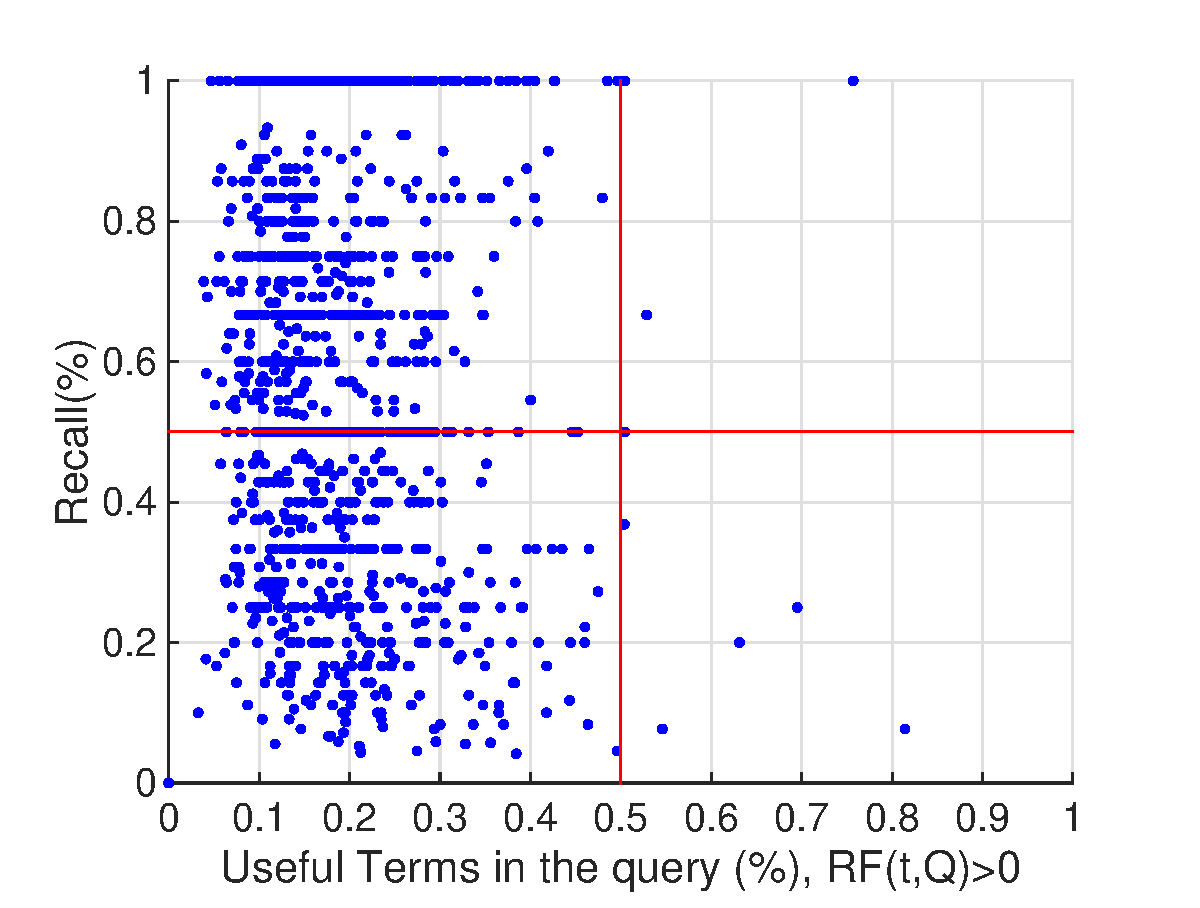
\includegraphics[width=5cm]{figs/greaterthan0-r.eps}} \hspace*{1.5cm} \subfigure[Useful terms: $ \{t|RF(t, Q)>RF(t_{+median})\} $]{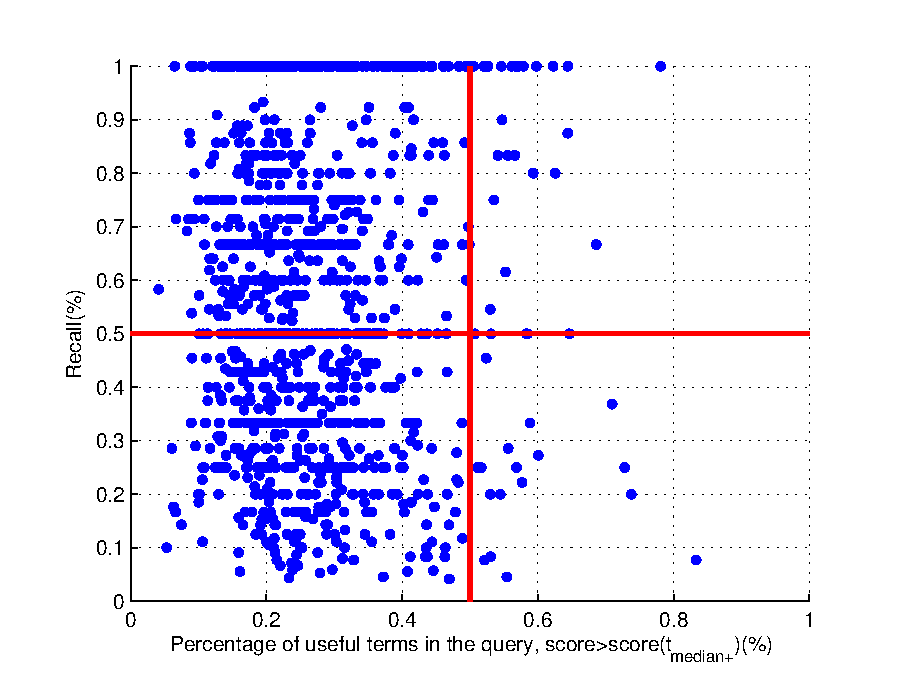
\includegraphics[width=5cm]{figs/greaterthanmedian-r.eps}}\\ \subfigure[{Useful terms: $ \{t|RF(t, Q)>1 \}$}]{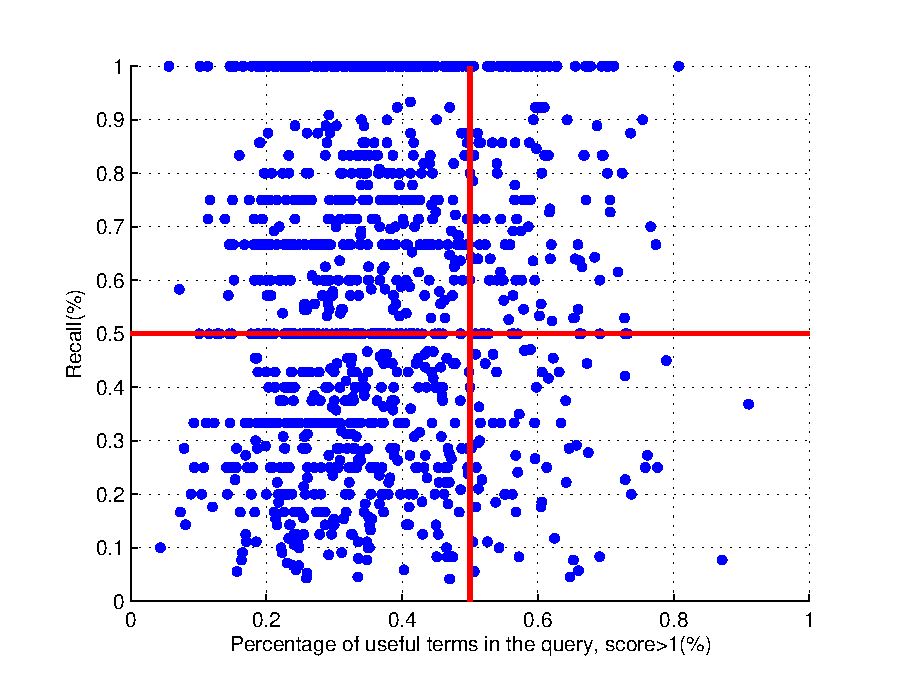
\includegraphics[width=5cm]{figs/greaterthan1-r.eps}} \hspace*{1.5cm} \subfigure[{Useful terms: top 100 high-scored terms}]{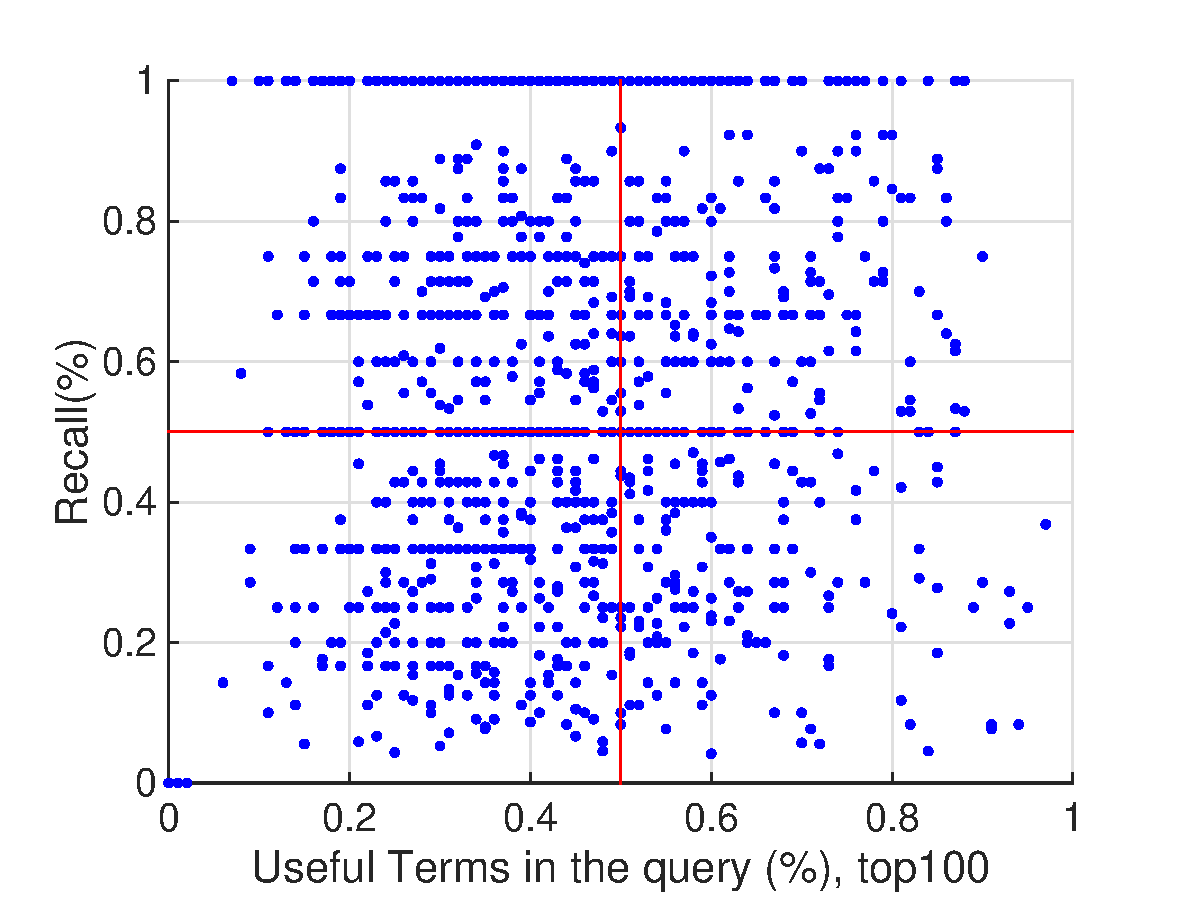
\includegraphics[width=5cm]{figs/top100-r.eps}}\\ \subfigure[{Useful terms:$ \{t|score(t,Q)>5 \}$}]{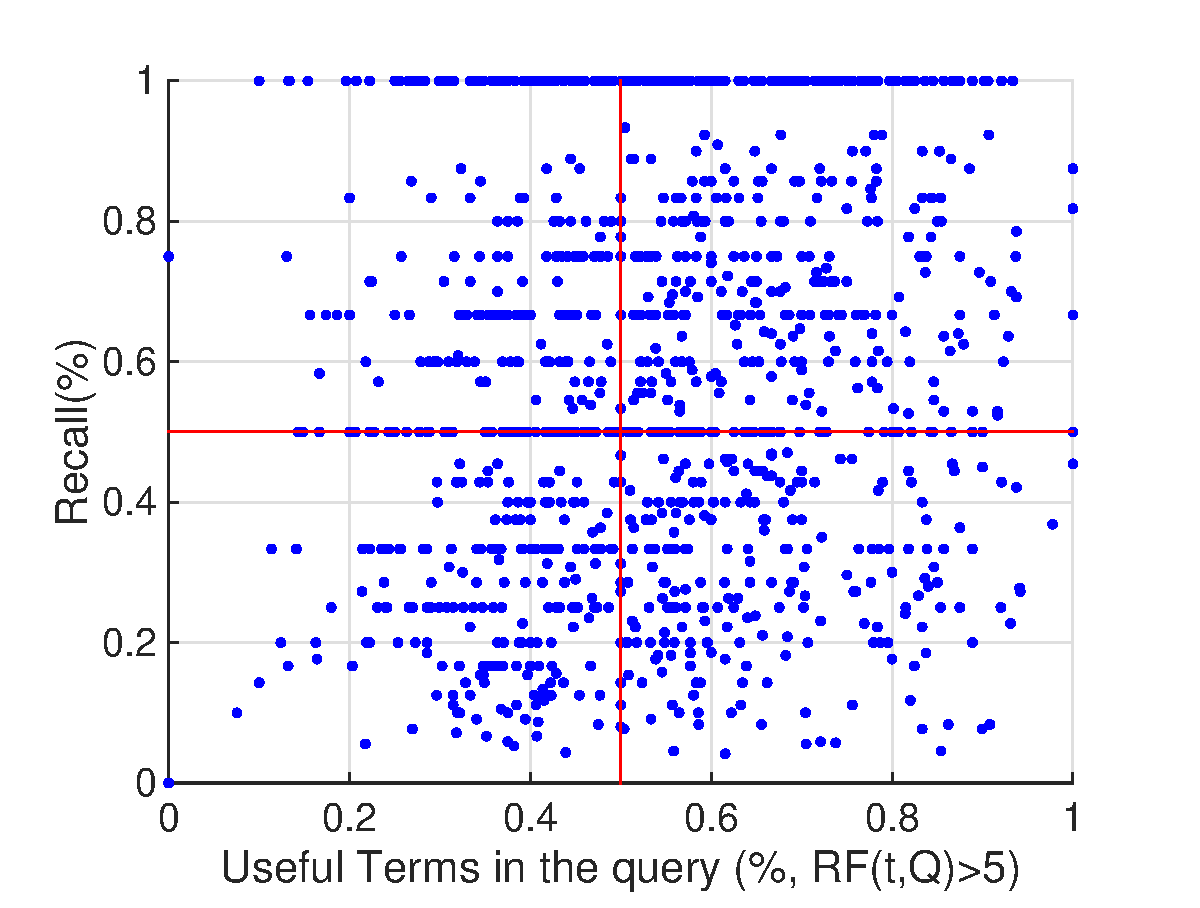
\includegraphics[width=5cm]{figs/greaterthan5-r.eps}} \hspace*{1.5cm} \subfigure[{Useful terms: $ \{t|RF(t, Q)>10\} $}]{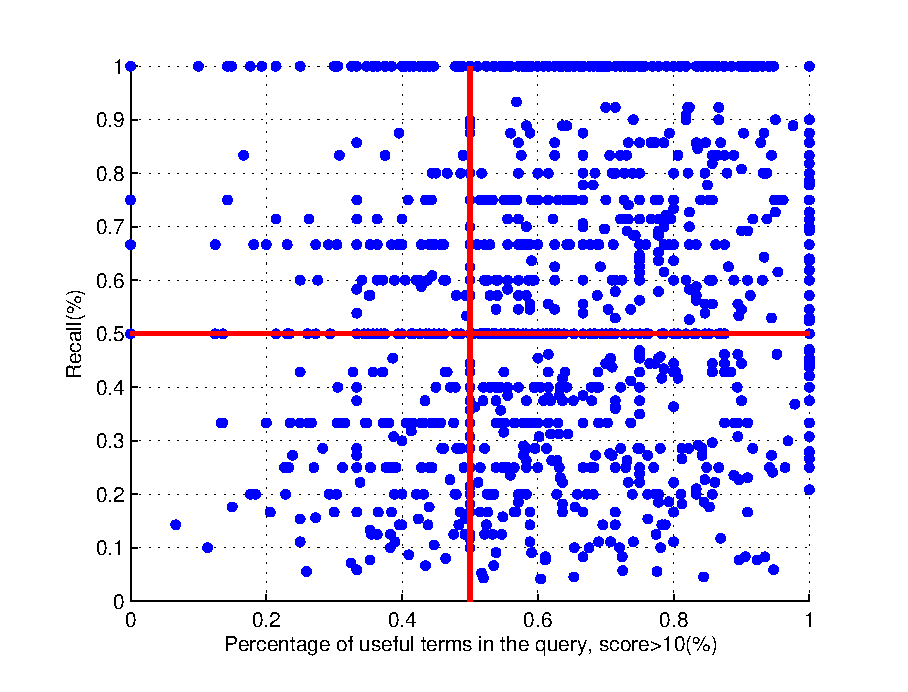
\includegraphics[width=5cm]{figs/greaterthan10-r.eps}}
\par\end{centering}

\protect\caption{Scatter plot of Recall vs. the overlap between useful terms and the the query.}
\label{fig:overlap-r}
\end{figure}
%%%%%%%%%%%%%%%%%%%%%%%%%%%%%%%%%%%%%%%%%%%%%%%%%%%%%%%%%%%%%%
%%%%%%%%%%%%%%%%%%%%%%%%%%%%%%%%%%%%%%%%%%%%%%%%%%%%%%%%%%%%%%
\begin{figure}[t!]
\begin{centering}
\subfigure[Useful terms: $ \{t|RF(t, Q)>0\} $]{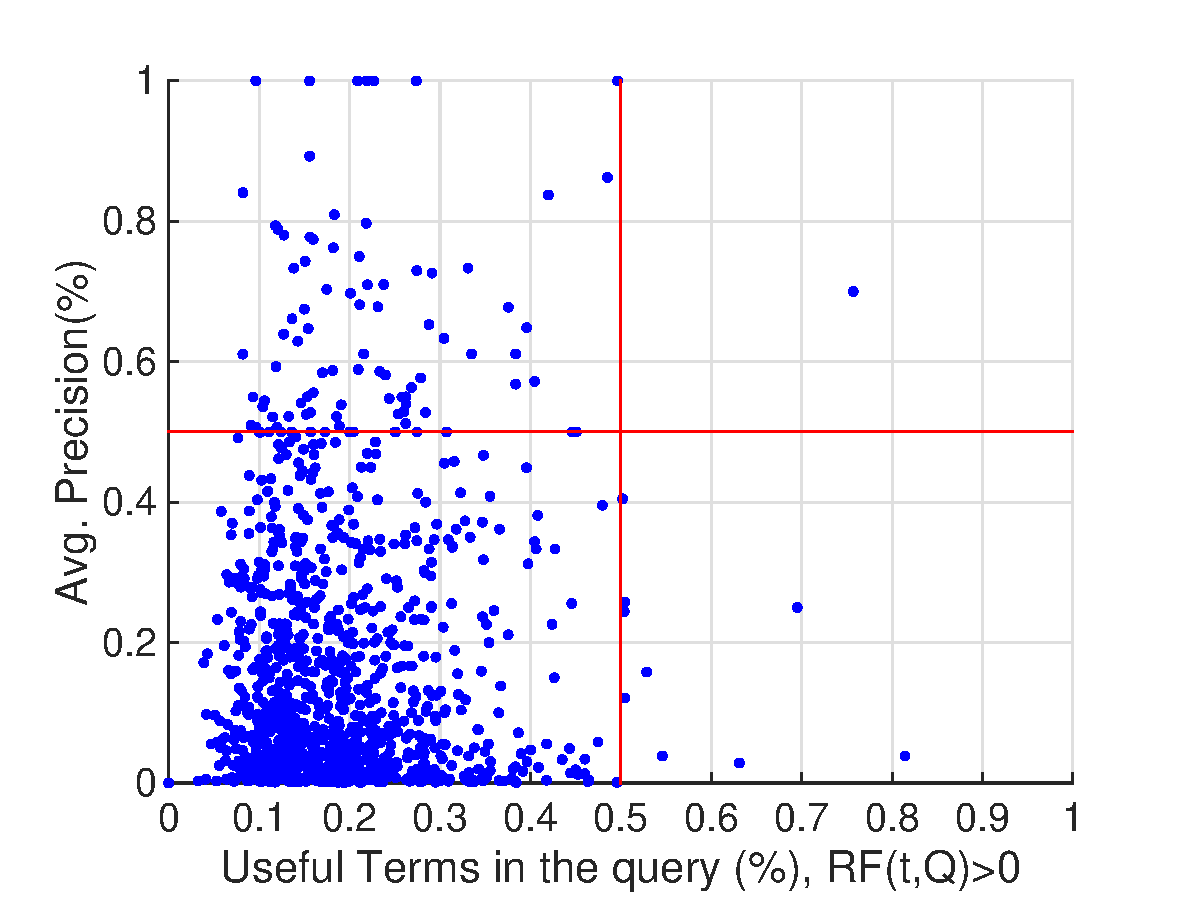
\includegraphics[width=5cm]{figs/greaterthan0-p}} \hspace*{1.5cm} \subfigure[Useful terms: $ \{t|RF(t, Q)>RF(t_{+median})\} $]{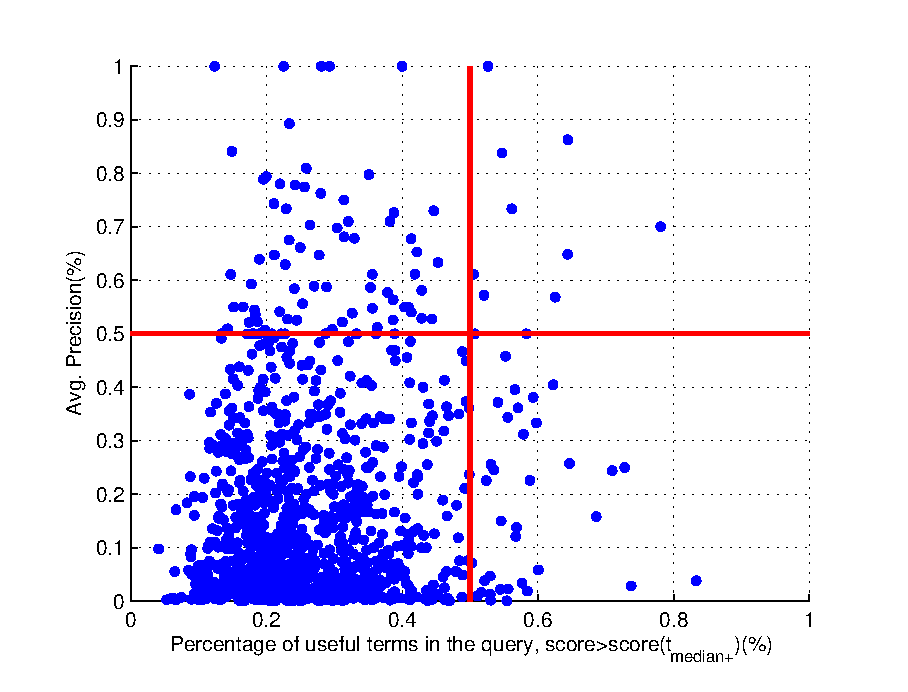
\includegraphics[width=5cm]{figs/greaterthammedian-p.eps}} \\[-2ex]% 
\subfigure[{Useful terms: $ \{t|RF(t, Q)>1 \}$}]{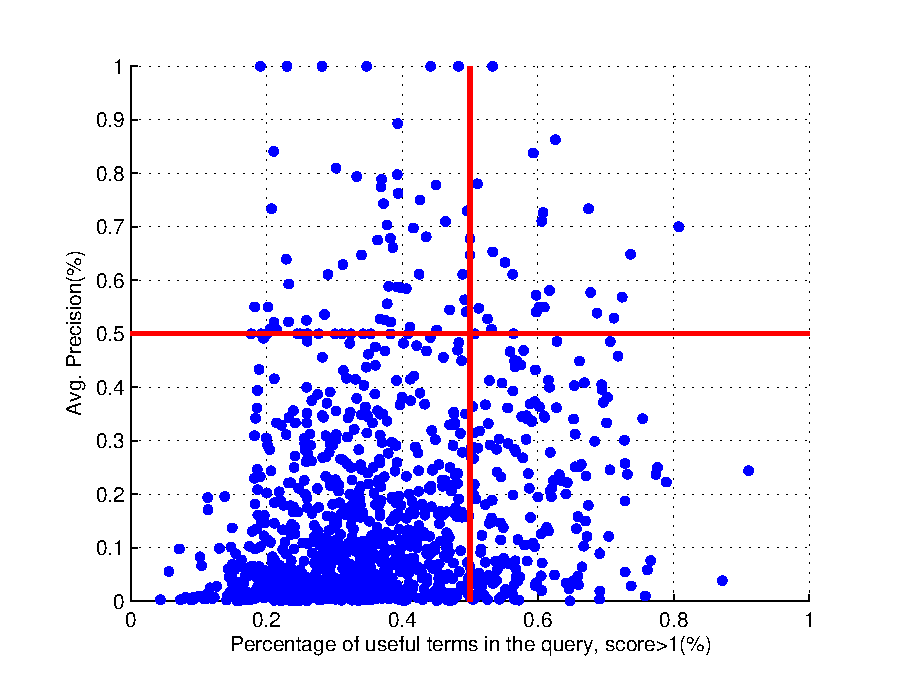
\includegraphics[width=5cm]{figs/greaterthan1-p.eps}} \hspace*{1.5cm} \subfigure[{Useful terms: top 100 high-scored terms}]{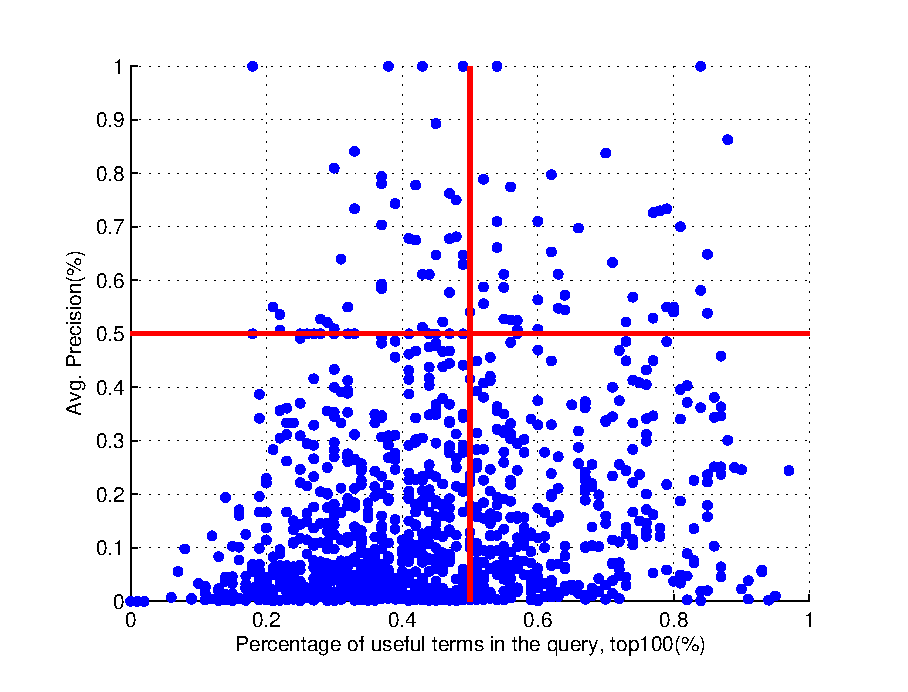
\includegraphics[width=5cm]{figs/top100-p.eps}}\\ [-2ex]%
\subfigure[{Useful terms:$ \{t|score(t,Q)>5 \}$}]{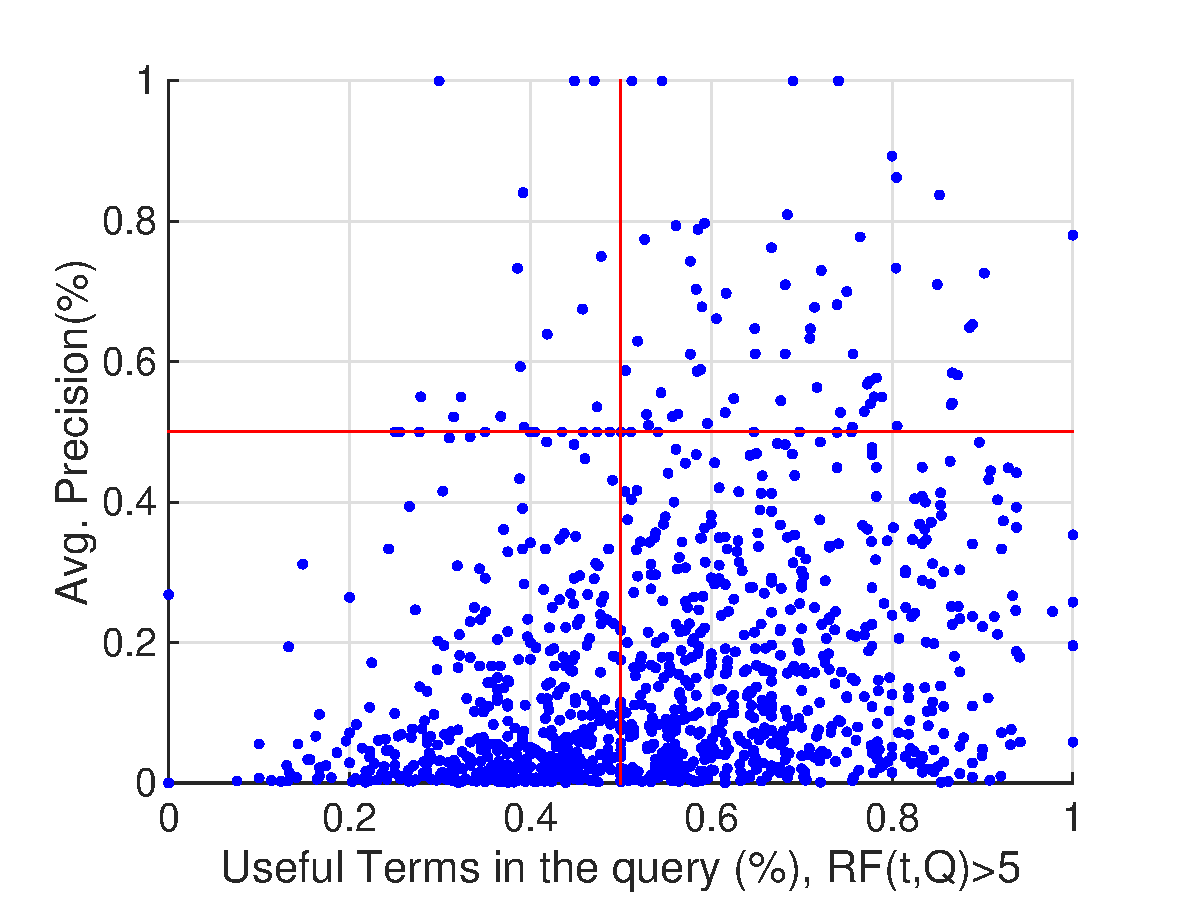
\includegraphics[width=5cm]{figs/greaterthan5-p.eps}} \hspace*{1.5cm} \subfigure[{Useful terms: $ \{t|RF(t, Q)>10\} $}]{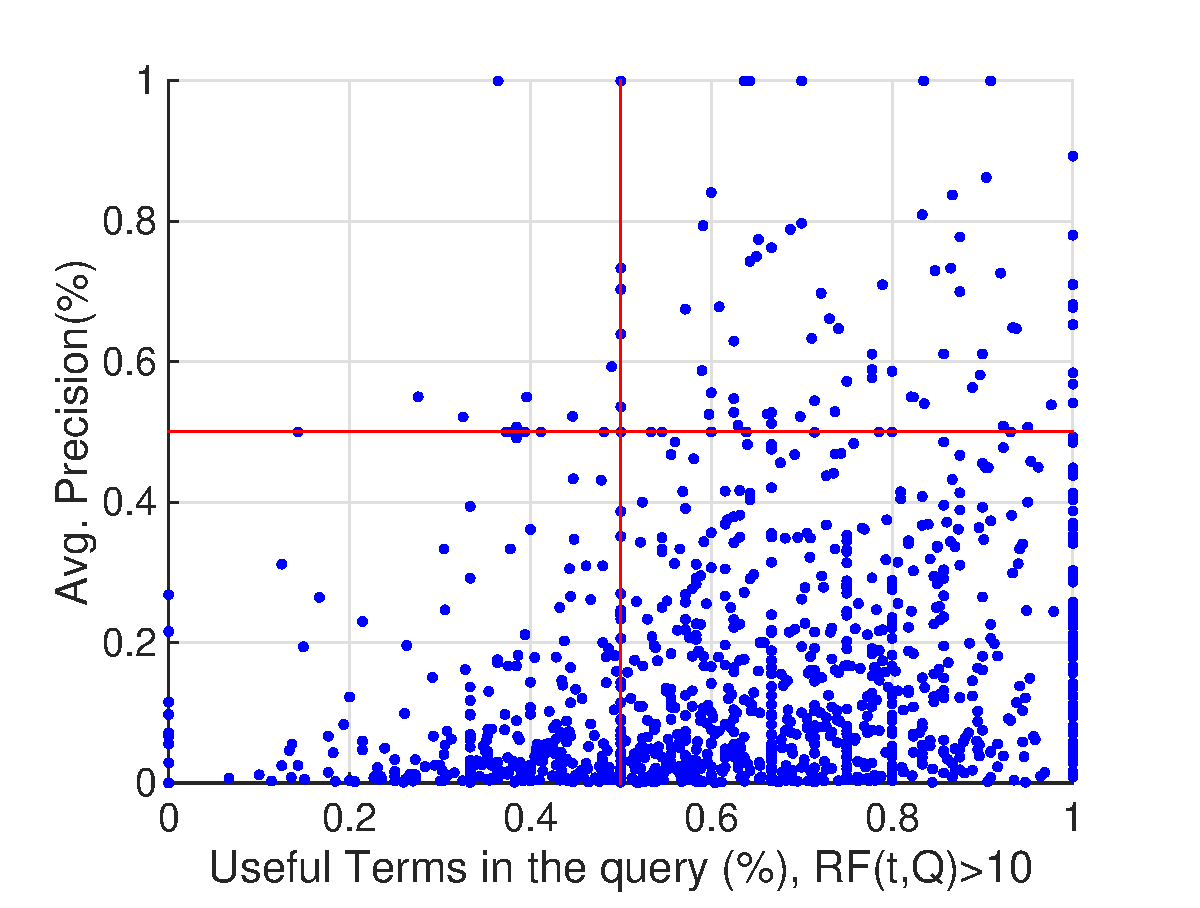
\includegraphics[width=5cm]{figs/greaterthan10-p.eps}}
\par\end{centering}

\protect\caption{Scatter plot of Average precision vs. the overlap between useful terms and the the query.}
\label{fig:overlap-p}
\end{figure}
%%%%%%%%%%%%%%%%%%%%%%%%%%%%%%%%%%%%%%%%%%%%%%%%%%%%%%%%%%%%%%
We expected to see a higher performance for the queries which contain more \textit{useful words} and a lower performance for the ones with less \textit{useful words}. However, unlike our first assumption, we could not find any correlation between the performance and the presence of \textit{useful words} in the query. The pattern for the recall is completely noisy while there is a very weak correlation between Average Precision and \textit{useful words} for top-scored words ($RF(t, Q)>10$). This experiment indicates that we should seek for reasons beyond the existence of the useful terms inside the query.  

Second, we check the term overlap with \textit{useful words} and \textit{noisy words} for TPs and FPs. Figure \ref{fig:usefulnoisy} shows that relevant patents have a higher term overlap with the \textit{useful words} while irrelevant patents have a higher term overlap with the \textit{noisy words}. This experiment shows that 
%%%%%%%%%%%%%%%%%%%%%%%%%%%%%%%%%%%%%%%%%%%%%%%%%%%%%%%%%%%%%%
\begin{figure}[t!]
\begin{centering}
\subfigure[Useful terms: $ \{t|RF(t, Q)>0\} $]{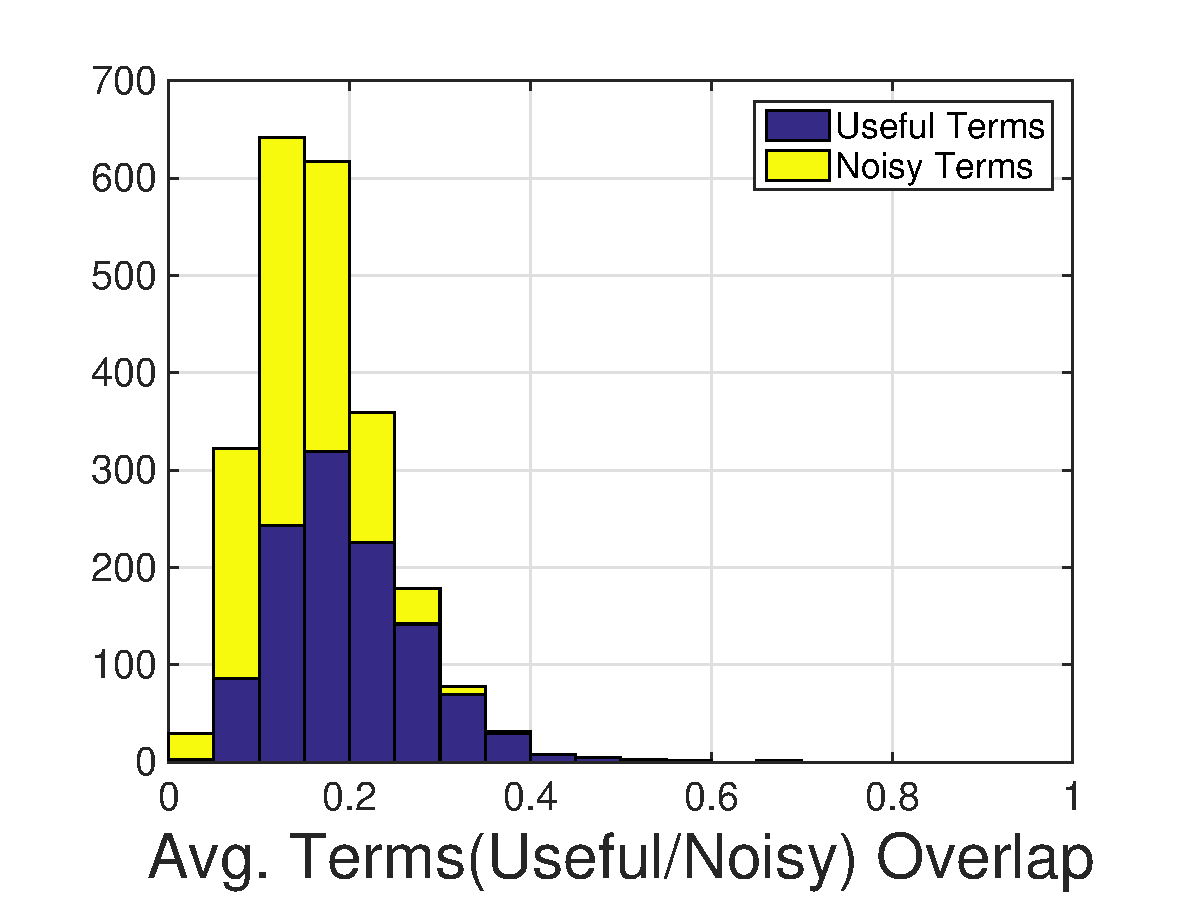
\includegraphics[width=5cm]{figs/stackedTPs.eps}} \hspace*{1.5cm} \subfigure[Useful terms: $ \{t|RF(t, Q)>RF(t_{+median})\} $]{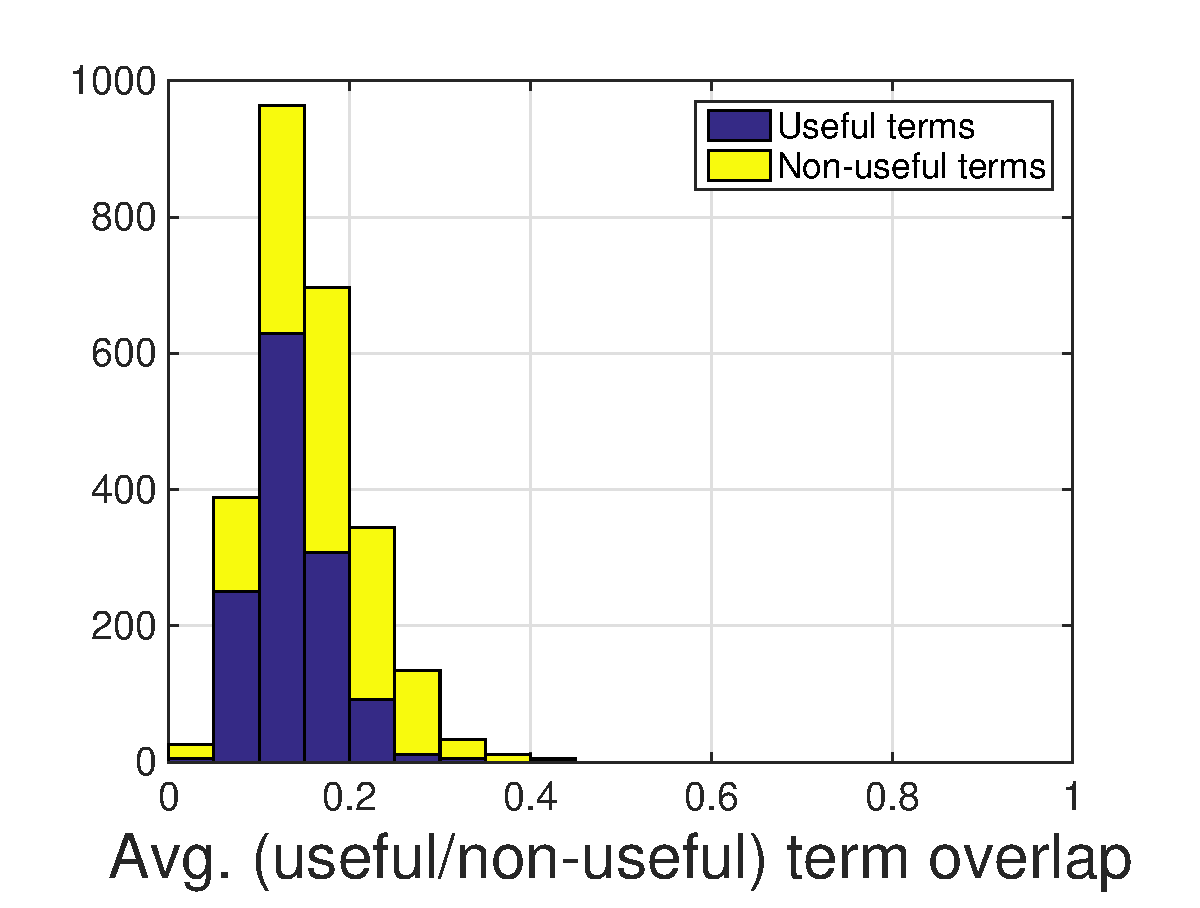
\includegraphics[width=5cm]{figs/stackedFPs.eps}} 
\par\end{centering}

\protect\caption{Scatter plot of Average precision vs. the overlap between useful terms and the the query.}
\label{fig:usefulnoisy}
\end{figure}
%%%%%%%%%%%%%%%%%%%%%%%%%%%%%%%%%%%%%%%%%%%%%%%%%%%%%%%%%%%%%%
%We hypothesized that a query, formulated by only the \textit{ useful terms}, is the best possible query we can make since they are all frequent in relevant patents but rare in irrelevant ones. 

\subsection{Oracular Query Formulation}
We empirically seek to evaluate the threshold $\tau$ on $RF(t,Q)$ (defined below) yielding the best oracular query.
We formulate two oracular queries. The first query is formulated by selecting terms in the top-100 documents:
\begin{equation}
Oracular \; Query = \{t \in top-100|RF(t, Q)>\tau\}   
 \label{eq:score}
\end{equation}
We formulate the second query by selecting terms that also occur in the reference patent query as follows:
% query based on the hypothesis that a patent query contains sufficient words matched with the relevant patents:
\begin{equation}
 Oracular \; Patent \; Query = \{t\in Q|RF(t, Q)>\tau\}   
 \label{eq:score}
\end{equation}
%\subsection{Discriminative Words}
%\label{sec:discriminative}
%
%\subsection{RF Optimal Query Formulation}
%\label{sec:formulation}

%%%%%%%%%%%%%%%%%%%%%%%%%%%%%%%%%%%%%%%%%%%%%%%%%%%%%%%%%%%%%%
%%%%%%%%%%%%%%%%%%%%%%%%% SECTION 3 %%%%%%%%%%%%%%%%%%%%%%%%%%
%%%%%%%%%%%%%%%%%%%%%%%%%%%%%%%%%%%%%%%%%%%%%%%%%%%%%%%%%%%%%%
\section{Query Reduction}

\subsection{Automated Reduction}
\subsection{Semi-automated Interactive Reduction}

\section{Section-based Analysis}

\section{Summary}
Same as the last chapter, summary what you discussed in this chapter and
be the bridge to next chapter.
